\documentclass{article}

\usepackage{neurips_2026}

\usepackage[utf8]{inputenc}
\usepackage[T1]{fontenc}
\usepackage{amsmath}
\usepackage{amsfonts}
\usepackage{amssymb}
\usepackage{booktabs}
\usepackage{graphicx}
\usepackage{hyperref}
\usepackage{microtype}
\usepackage[numbers]{natbib}
\usepackage{xcolor}

\emergencystretch=2em
\setlength{\textfloatsep}{8pt plus 1pt minus 2pt}
\setlength{\floatsep}{6pt plus 1pt minus 1pt}
\setlength{\intextsep}{6pt plus 1pt minus 1pt}

\title{Warm-Start Diffusion for Low-Resolution Probabilistic ERA5 Weather Forecasting}

\author{%
  Kabir Vats (Team 43)\\
  \small Code: \url{https://github.com/kabir-vats/Warm-Start-Diffusion}
}

\newcommand{\optionalfig}[4]{%
\begin{figure}[t]
    \centering
    \IfFileExists{#1}{%
        \includegraphics[width=0.92\linewidth,height=0.30\textheight,keepaspectratio]{#1}%
    }{%
        \fbox{\begin{minipage}[c][0.72in][c]{0.92\linewidth}
            \centering
            \footnotesize \textbf{Placeholder figure.} #4
        \end{minipage}}%
    }
    \caption{#3}
    \label{#2}
\end{figure}}

\begin{document}

\maketitle

\begin{abstract}
Probabilistic weather forecasting needs both strong forecast scores and physically reasonable samples. In this project, I test a simple hybrid for low-resolution ERA5-MINI: first a U-Cast-style Monte Carlo dropout U-Net makes a forecast, then an EDM diffusion model is warm-started from that forecast and denoises only at lower noise levels. Averaged across evaluated timestamps, U-Cast gets CRPS/RMSE of 86.798/202.97, cold-start diffusion gets 89.26/211.03, warm-start diffusion improves this to 85.23/201.94, and fine-tuned warm-start diffusion reaches 84.98/201.59. The result supports the main idea: CRPS training is good at forecast placement, while diffusion is useful as a more physical low-noise refiner.
\end{abstract}

\section{Introduction}

Weather forecasting is a hard probabilistic generation problem because the outputs need to score well and still look like actual weather. In this project, I use ERA5-MINI, a coarse $64\times32$ global ERA5/WeatherBench2-style grid, so that I can test the idea without needing full operational-scale training. The model predicts 12-hour transitions from two previous states and is evaluated over 15 autoregressive steps. This setting is small, but it still keeps the main pieces that matter here: global spatial structure, autoregressive error growth, uncertainty, and the question of whether samples look physically plausible.

The main issue is the tradeoff between direct probabilistic training and diffusion generation. CRPS-trained systems such as FGN, AIFS-CRPS, and U-Cast optimize forecast skill directly and are efficient at inference \citep{alet2025fgn,lang2026aifscrps,cachay2026ucast}. Diffusion models learn a denoising generative process and often produce better spatial structure, but cold-start sampling begins far from the data manifold and requires many denoising evaluations \citep{ho2020ddpm,price2025gencast,brenowitz2025cbottle}. So I test whether diffusion is more useful as a local refiner: start from a strong CRPS forecast, add controlled noise, and denoise only the lower-noise tail of the EDM schedule.

The main pieces of the project are: (1) a U-Cast-style ERA5-MINI baseline trained with weighted MAE then weighted CRPS and Monte Carlo dropout; (2) a conditional EDM baseline with the same Dhariwal-style U-Net backbone; (3) a warm-start sampler and fine-tuning setup using the CRPS model as the proposal; and (4) evaluation using aggregate CRPS/RMSE, lead-time skill curves, warm-start-step ablation, and spectra. The observed ordering is fine-tuned warm-start EDM $>$ warm-start EDM $>$ U-Cast-style CRPS $\gg$ cold-start EDM. The effects are small, but they are consistent across the aggregate table and the lead-time plot, and they support the hypothesis that CRPS gives strong forecast placement while diffusion supplies a more physical local prior.

\section{Related Work}

GraphCast showed that neural models can make skillful medium-range forecasts from ERA5 \citep{lam2023graphcast}, while ERA5 and WeatherBench2 provide the reanalysis and benchmark context for this project \citep{hersbach2020era5,rasp2024weatherbench2}. I do not try to reproduce a full GraphCast-style system here. Instead, I use a small ERA5-MINI setting whose variables follow the parsimonious modeling spirit of DLWP-HPX \citep{karlbauer2024healpix}. DLWP-HPX uses $Z_{1000}$, $Z_{500}$, $Z_{300}-Z_{700}$ thickness, $T_{2m}$, $T_{850}$, $TCWV$, and $Z_{250}$; here I keep $Z_{300}$ and $Z_{700}$ separate, giving eight predicted channels. This is a useful middle ground: the task is much cheaper than full weather prediction, but it still includes vertical structure, surface temperature, and moisture.

Proper scoring rules such as CRPS are standard for probabilistic forecasting \citep{gneiting2007proper}. U-Cast is the closest baseline: a simple U-Net is pretrained deterministically, fine-tuned with CRPS, and sampled using Monte Carlo dropout \citep{cachay2026ucast,gal2016dropout}. Diffusion models instead reverse a noise process \citep{ho2020ddpm}; I use an EDM formulation \citep{karras2022edm} and a Dhariwal/Nichol U-Net family \citep{dhariwal2021diffusion,ronneberger2015unet}. Weather diffusion systems such as GenCast and cBottle motivate diffusion for sample quality \citep{price2025gencast,brenowitz2025cbottle}, while fast sampling and warm-start work motivate avoiding unnecessary high-noise denoising when a strong conditional proposal is available \citep{salimans2022progressive,scholz2025warmstarts}. This project focuses on that specific gap: direct CRPS training gives strong scalar skill, but diffusion may add a spectral/sample-quality prior if it is used only where it is most reliable.

This is also why the comparison is not just ``diffusion versus non-diffusion.'' A cold-start diffusion model is a hard baseline because it has to learn the whole conditional generation path from high noise. A U-Cast-style model is a hard baseline in the other direction because it is trained directly for the probabilistic score. The warm-start model is meant to test whether these two strengths are actually complementary, rather than choosing one family over the other.

\section{Method}

\paragraph{Forecasting setup and architecture.}
Let $x_t\in\mathbb{R}^{C\times H\times W}$ be the normalized ERA5-MINI state, with $C=8$ channels and $(H,W)=(64,32)$:
\[
\{T_{2m}, Z_{250}, Z_{300}, Z_{500}, Z_{700}, Z_{1000}, T_{850}, TCWV\}.
\]
Inputs are $(x_{t-12h},x_t)$ plus land-sea mask, surface geopotential, and sine/cosine day/year progress. Losses use latitude weighting by $\cos(\phi)$ so that polar grid cells do not dominate the objective. The runs train on 1979--2019 slices and evaluate in validation mode with up to 128 samples and 10 ensemble predictions per initial condition. The metrics are reported in the same evaluation units for all models, so the comparison is relative rather than a claim about operational absolute error. All variants use the same Dhariwal-style convolutional U-Net: 256 base channels, channel multipliers $[1,2,4]$, residual prediction, dropout $0.1$, attention at lower resolutions, and circular longitude padding.

\paragraph{U-Cast-style baseline.}
The deterministic stage predicts a residual update and minimizes weighted MAE,
\[
\mathcal{L}_{\mathrm{WMAE}}
=
\mathbb{E}\sum_{c,i,j} w_{c,i,j}
\left| f_\theta(x_{t-12h},x_t)_{c,i,j}-x_{t+12h,c,i,j}\right|.
\]
The probabilistic stage enables dropout and minimizes weighted ensemble CRPS:
\[
\mathrm{CRPS}(\{y^{(m)}\},x)=
\frac{1}{M}\sum_m\lVert y^{(m)}-x\rVert_1
-
\frac{1}{2M^2}\sum_{m,n}\lVert y^{(m)}-y^{(n)}\rVert_1.
\]
The main CRPS model uses two training ensemble members and 10 Monte Carlo dropout samples at evaluation. This same model also supplies the warm-start proposal for diffusion.

\paragraph{Cold-start EDM.}
The diffusion baseline follows EDM \citep{karras2022edm}. For context $c=(x_{t-12h},x_t)$, sample $\sigma$ and $\epsilon\sim\mathcal{N}(0,I)$, corrupt the target as $z=x+\sigma\epsilon$, and train $D_\theta$ with
\[
\mathcal{L}_{\mathrm{EDM}}
=
\mathbb{E}_{x,c,\sigma,\epsilon}
\lambda(\sigma)\lVert D_\theta(x+\sigma\epsilon,c,\sigma)-x\rVert_2^2.
\]
The baseline uses $\sigma_{\min}=0.002$, $\sigma_{\max}^{\mathrm{inf}}=800$, $\rho=7$, 20 sampler steps, $P_{\mathrm{mean}}=-1.6$, $P_{\mathrm{std}}=1.6$, weighted MSE, batch size 128, and 10k training steps. This model has realistic spectra but weaker direct skill, likely because the same denoiser has to handle both high-noise generation and low-noise forecast correction.

\paragraph{Warm-start EDM.}
Warm-start diffusion initializes from a CRPS forecast rather than from high noise. If $\hat{x}^{\mathrm{UC}}_{t+h}\sim q_\psi(x_{t+h}\mid x_{t-12h},x_t)$, I start the sampler from
\[
z_{\sigma_K}=\hat{x}^{\mathrm{UC}}_{t+h}+\sigma_K\epsilon,\qquad \epsilon\sim\mathcal{N}(0,I),
\]
then run the low-noise tail $z_{\sigma_K}\to\cdots\to z_{\sigma_0}$. The best inference setup uses U-Cast guidance, 6 warm-start steps out of a 20-step EDM schedule, warm-start dropout, and 10 predictions. I also fine-tune the diffusion model for this regime, using $P_{\mathrm{mean}}=-3$, $P_{\mathrm{std}}=1$, $\sigma_{\max}^{\mathrm{inf}}=400$, and per-sigma loss logging.

\optionalfig{figures/warm_start_method.png}{fig:warm-start-pipeline}{Warm-start diffusion pipeline. The autoregressive CRPS model proposes an initial forecast, partial noise is added, and the diffusion model refines the noised forecast while conditioning on the initial weather state.}{Save the attached warm-start method diagram as \texttt{figures/warm\_start\_method.png}.}

\paragraph{Baselines and metrics.}
The comparison includes deterministic WMAE U-Net, U-Cast-style WCRPS U-Net, cold-start EDM, warm-start EDM, and fine-tuned warm-start EDM. I focus on normalized CRPS, RMSE, lead-time skill curves, the warm-start step ablation, and energy spectra.

At inference time, the difference between the three probabilistic systems is fairly concrete. The U-Cast-style model samples the same network repeatedly with dropout enabled. The cold-start EDM model starts from the usual high-noise EDM initialization and runs the full 20-step sampler. The warm-start model first draws a U-Cast forecast, adds noise at an intermediate EDM level, and then runs only the last few denoising steps. This means the warm-start model is not asking diffusion to invent the whole atmospheric state. It asks diffusion to make a local correction to a forecast that is already plausible.

\section{Results and Analysis}

\paragraph{Experimental details.}
All main experiments use 12-hour resolution, window size 2, 15-step rollout, 256 model channels, $[1,2,4]$ channel multipliers, residual prediction, dropout $0.1$, and latitude-weighted losses. The U-Cast-style baseline enables inference dropout. Cold-start diffusion uses 20 EDM steps with $\sigma_{\min}=0.002$, $\sigma_{\max}^{\mathrm{inf}}=800$, and no warm start. Warm-start diffusion uses the same EDM model with U-Cast guidance, 6 warm-start steps, and 10 predictions. The CRPS model is initialized from the deterministic WMAE checkpoint.

Table~\ref{tab:skill} reports the aggregate metrics averaged across all evaluated timestamps. I leave out the deterministic MAE-only baseline because I do not have the corresponding aggregate CRPS/RMSE values for that model.

For the lead-time plot, I use the U-Cast-style model as the baseline and show percent difference relative to that model. This makes the plot easier to read because the raw metric values are close, but the ordering is what matters. Positive values mean worse than U-Cast, while negative values mean better than U-Cast. This is also why the diffusion baseline is useful even though it performs worse: it shows that the gain is not simply from adding diffusion compute, but from using diffusion in the right noise regime.

\begin{table}[t]
    \centering
    \caption{Aggregate forecast skill averaged across all evaluated timestamps. Lower is better for both metrics.}
    \label{tab:skill}
    \small
    \begin{tabular}{@{}p{0.27\linewidth}p{0.13\linewidth}p{0.13\linewidth}p{0.35\linewidth}@{}}
        \toprule
        Model & CRPS $\downarrow$ & RMSE $\downarrow$ & Notes \\
        \midrule
        U-Cast-style CRPS & 86.798 & 202.97 & Strong direct probabilistic baseline. \\
        Cold-start EDM & 89.26 & 211.03 & Worse skill, but more physical spectra. \\
        Warm-start EDM & 85.23 & 201.94 & Best non-fine-tuned hybrid. \\
        Fine-tuned warm-start EDM & 84.98 & 201.59 & Best overall aggregate skill. \\
        \bottomrule
    \end{tabular}
\end{table}

The completed runs show the ordering fine-tuned warm-start EDM $>$ warm-start EDM $>$ U-Cast-style CRPS $\gg$ cold-start EDM on the aggregate metrics. Relative to U-Cast, warm start improves CRPS by 1.57 and RMSE by 1.03, while fine-tuned warm start improves CRPS by 1.82 and RMSE by 1.38. In percentage terms, the fine-tuned warm-start model improves the U-Cast CRPS by about 2.1\% and RMSE by about 0.7\%. These are not huge gains, but they are meaningful in this setting because U-Cast is already a strong direct probabilistic baseline. Cold-start EDM is much worse on direct skill, supporting the view that the full high-to-low-noise denoising task is not well matched to this forecast metric. Warm start helps because the CRPS model supplies the forecast placement and diffusion only has to make a local correction near the data manifold.

\optionalfig{figures/lead_time_skill.png}{fig:skill-curves}{Lead-time CRPS percent difference from the U-Cast-style baseline for 2m temperature. Cold-start diffusion is worse than the baseline, while warm start and fine-tuned warm start improve consistently across lead times.}{Save the attached CRPS/RMSE-over-time plot as \texttt{figures/lead\_time\_skill.png}.}

\paragraph{Lead-time and physical diagnostics.}
The lead-time curve in Figure~\ref{fig:skill-curves} gives a more useful view than the aggregate table alone. For 2m temperature CRPS, cold-start diffusion is worse than the U-Cast baseline at every shown lead time, while both warm-start variants are better. The gap is largest at earlier lead times and narrows somewhat later in the rollout, but the sign of the effect stays consistent. This matters because it suggests the result is not coming from one lucky forecast horizon.

The energy spectrum diagnostic is central. For $Z_{250}$, U-Cast has excess high-wavenumber power relative to the ground truth, while diffusion and warm start track the ground-truth decay more closely. This explains the apparent tension in the scalar metrics: diffusion alone is not the best forecaster, but it learns a useful prior over spatial structure. Warm-start diffusion benefits from both sides: U-Cast supplies large-scale forecast placement, and low-noise EDM refinement nudges samples toward a more realistic atmospheric manifold.

\optionalfig{figures/spectrum_z250.png}{fig:spectra}{Energy spectrum for $Z_{250}$. U-Cast over-amplifies high wavenumbers, whereas diffusion and warm start are closer to the ground-truth spectral slope.}{Save the attached $Z_{250}$ spectrum as \texttt{figures/spectrum\_z250.png}.}

\paragraph{Why warm start helps.}
The result is best understood as a division of labor. The CRPS model solves forecast placement; diffusion supplies a sample-manifold prior. Cold-start diffusion asks one model to do both from high noise. Warm start instead asks EDM to repair an already plausible forecast, and fine-tuning further specializes the denoiser to the low-noise regime actually used at inference. Figure~\ref{fig:warm-start-ablation} supports this interpretation. Six warm-start denoising steps gives the best CRPS/RMSE tradeoff. Fewer steps do not give the diffusion model enough room to refine the forecast, while too many steps move the sampler back toward the weaker cold-start behavior. This matches the high-noise/low-noise tradeoff that motivated the method.

\begin{table}[t]
    \centering
    \caption{Warm-start denoising step ablation. Six steps is best for both aggregate CRPS and RMSE.}
    \label{tab:warm-start-steps}
    \small
    \begin{tabular}{ccc}
        \toprule
        Warm-start steps & CRPS $\downarrow$ & RMSE $\downarrow$ \\
        \midrule
        3 & 86.700 & 202.684 \\
        5 & 85.747 & 201.958 \\
        6 & 85.233 & 201.936 \\
        7 & 85.510 & 202.901 \\
        8 & 86.537 & 205.109 \\
        10 & 88.232 & 208.617 \\
        \bottomrule
    \end{tabular}
\end{table}

\begin{figure}[t]
    \centering
    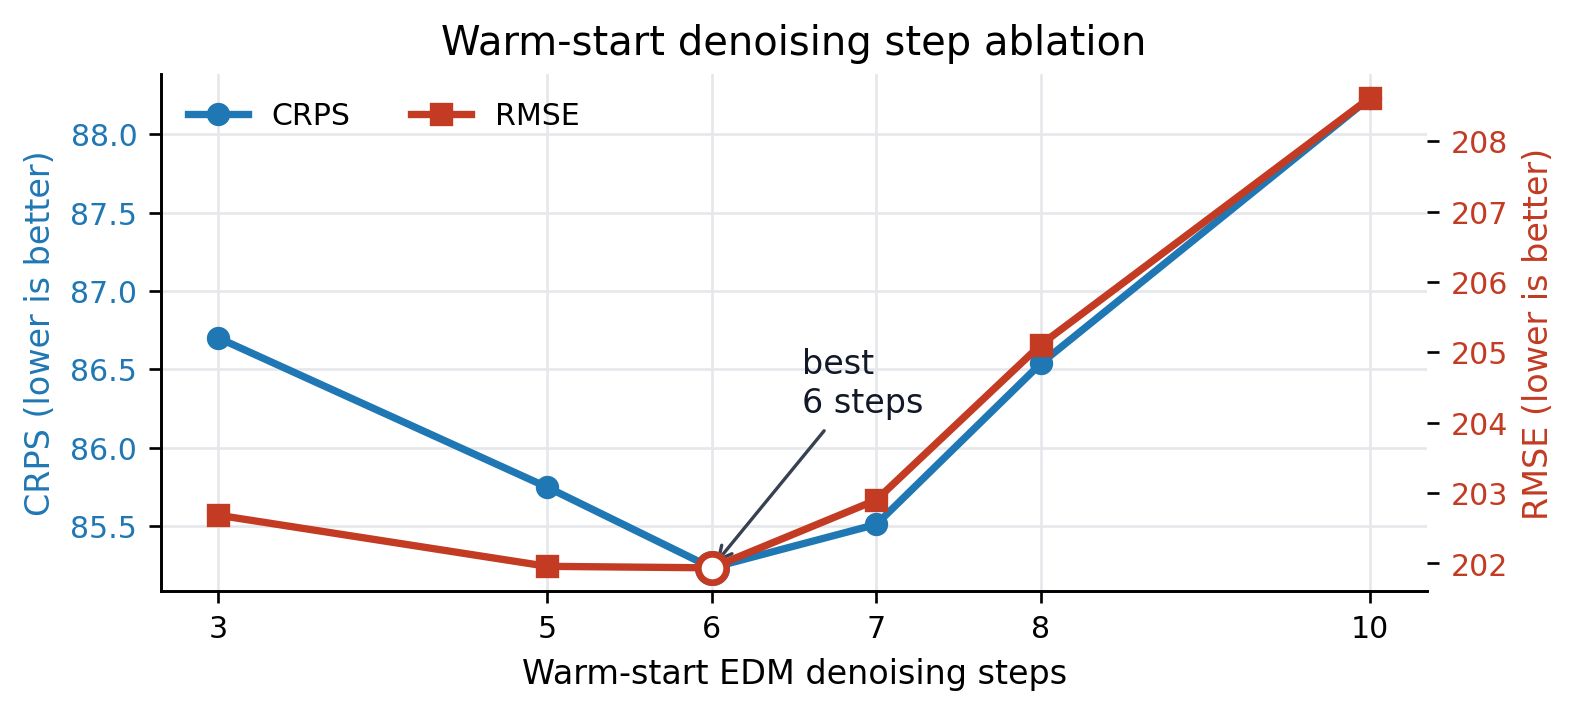
\includegraphics[width=0.78\linewidth]{figures/warm_start_steps_ablation.png}
    \caption{Warm-start step ablation. Six denoising steps gives the lowest CRPS and RMSE; both shorter and longer warm-start trajectories degrade the aggregate metrics.}
    \label{fig:warm-start-ablation}
\end{figure}

\section{Limitations}

There are a few important limitations. ERA5-MINI is deliberately low resolution, so this should not be read as evidence about operational-resolution forecasting. The comparison is also not compute-normalized: diffusion uses multiple U-Net evaluations per sample, while U-Cast is much cheaper. The result also does not include every diagnostic I would want in a larger study, especially reliability diagrams, spread-error curves, and rollout maps for several variables. Finally, the current analysis is strongest for aggregate skill and spectra; future work should test higher resolution, more variables, and stricter test-set evaluation.

\section{Conclusion}

Overall, this project suggests that diffusion is more useful for this setting when it starts from a strong direct forecast rather than from pure noise. U-Cast gives strong direct skill, cold-start EDM gives a more physical prior but weaker metrics, and warm-start EDM combines the two to give the best observed performance. The broader lesson is that forecast skill and physical sample quality are related but not identical. Warm-start diffusion is a practical way to combine CRPS-trained forecasting with diffusion-based refinement, and fine-tuning the denoiser for the warm-start regime appears most promising.

\clearpage
\bibliographystyle{plainnat}
\bibliography{refs}

\end{document}
